\documentclass[11pt]{article}

\usepackage[T1]{fontenc}
\usepackage[utf8]{inputenc}
\usepackage{lmodern}
\usepackage{microtype}
\usepackage[margin=1in]{geometry}
\usepackage{amsmath,amssymb,amsthm,mathtools}
\usepackage{stmaryrd}
\usepackage{booktabs,longtable,array,tabularx}
\usepackage{enumitem}
\usepackage{xcolor}
\usepackage{listings}
\usepackage{tikz}
\usetikzlibrary{arrows.meta,positioning,fit,calc}
\usepackage{hyperref}
\usepackage[nameinlink,noabbrev]{cleveref}
\usepackage{fancyhdr}
\usepackage{lastpage}

\definecolor{BusyBlue}{HTML}{174A7E}
\definecolor{BusyTeal}{HTML}{0B6E69}
\definecolor{BusyRed}{HTML}{9B2C2C}
\definecolor{BusyGray}{HTML}{4A5568}
\definecolor{CodeBg}{HTML}{F6F8FA}
\definecolor{CodeRule}{HTML}{D0D7DE}

\hypersetup{
  colorlinks=true,
  linkcolor=BusyBlue,
  citecolor=BusyTeal,
  urlcolor=BusyBlue,
  pdftitle={Contender 35: Transfinite Metalanguage Reflection over Tree Ordinals},
  pdfauthor={Research proposal for the BusyLean project}
}

\pagestyle{fancy}
\fancyhf{}
\lhead{BusyLean Contender 35}
\rhead{Transfinite metalanguage reflection}
\cfoot{\thepage\ of \pageref{LastPage}}
\setlength{\headheight}{14pt}

\lstdefinelanguage{Lean}{
  morekeywords={def,theorem,lemma,inductive,structure,namespace,end,open,import,
    where,match,with,if,then,else,let,in,fun,by,exact,have,show,from,do,pure,
    private,partial,unsafe,noncomputable,deriving,instance,abbrev,opaque},
  sensitive=true,
  morecomment=[l]{--},
  morecomment=[s]{/-}{-/},
  morestring=[b]"
}
\lstset{
  language=Lean,
  basicstyle=\ttfamily\footnotesize,
  keywordstyle=\color{BusyBlue}\bfseries,
  commentstyle=\color{BusyGray}\itshape,
  stringstyle=\color{BusyTeal},
  backgroundcolor=\color{CodeBg},
  frame=single,
  rulecolor=\color{CodeRule},
  framesep=5pt,
  breaklines=true,
  breakatwhitespace=false,
  columns=fullflexible,
  keepspaces=true,
  showstringspaces=false,
  tabsize=2,
  numbers=left,
  numberstyle=\tiny\color{BusyGray},
  numbersep=8pt,
  xleftmargin=1.7em,
  framexleftmargin=1.2em,
  literate=
    {Γ}{{$\Gamma$}}1
    {Σ}{{$\Sigma$}}1
    {ρ}{{$\rho$}}1
    {←}{{$\leftarrow$}}1
    {→}{{$\to$}}1
    {∀}{{$\forall$}}1
    {∈}{{$\in$}}1
    {≤}{{$\le$}}1
    {▸}{{$\triangleright$}}1
    {⟨}{{$\langle$}}1
    {⟩}{{$\rangle$}}1
}

\newtheorem{theorem}{Theorem}[section]
\newtheorem{proposition}[theorem]{Proposition}
\newtheorem{lemma}[theorem]{Lemma}
\newtheorem{corollary}[theorem]{Corollary}
\theoremstyle{definition}
\newtheorem{definition}[theorem]{Definition}
\newtheorem{remark}[theorem]{Remark}
\newtheorem{designprinciple}[theorem]{Design principle}

\newcommand{\CTree}{\mathsf{CTree}}
\newcommand{\Nat}{\mathbb{N}}
\newcommand{\Op}{\mathcal{O}}
\newcommand{\MOp}{\mathcal{M}}
\newcommand{\Lang}{\mathsf{Lang}}
\newcommand{\MetaLang}{\mathsf{MetaLang}}
\newcommand{\Fthirtyfour}{F_{34}}
\newcommand{\Fthirtyfive}{F_{35}}
\newcommand{\Cthirtyfour}{C_{34}}
\newcommand{\Cthirtyfive}{C_{35}}
\newcommand{\Lean}{\textsc{Lean}}
\newcommand{\code}[1]{\texttt{#1}}
\newcommand{\StatusText}{The exact Lean~4.34.0 repository build succeeded at commit \code{f08df5f2a4cb} in GitHub Actions run \code{38440600428}; the verification branch's full name and complete commit hash are recorded in \code{VERIFICATION.md}.  With the accepted baseline precompiled, the measured module times were 0.53 seconds for \code{TreeLanguage4}, 0.33 seconds for \code{Contender35}, and 0.33 seconds for \code{Comparison35}.  The axiom report is exactly within the repository allowance: the evaluator uses no axioms; the tree closures use \code{propext}; the number and comparison theorem use \code{propext} and \code{Quot.sound}.  The dependency closure contained 5,534 constants and none of the thirty forbidden contender constants 5 through 34.}

\title{\textbf{Contender 35: Transfinite Metalanguage Reflection\\over Tree Ordinals}}
\author{A research proposal for the BusyLean project}
\date{13 October 2026}

\begin{document}
\maketitle

\begin{abstract}
The accepted BusyLean Contender~34 iterates a first-order language-closure
operator along a countable tree ordinal.  This report proposes a qualitatively
stronger construction, Contender~35, by raising the closure mechanism itself
one functional type.  A new simply typed metalanguage has a primitive
\[
  \mathsf{lift} : (\CTree\to\CTree)\to\CTree\to\CTree,
\]
so programs can construct tree transformers, pass them to a lower-level
language-closure operator, and continue computing with the resulting trees.
The total semantic interpreter, raw syntax, type checker, and finite program
enumerator are all defined constructively in Lean.  The induced metalanguage
closure is then iterated by structural recursion along Contender~34's own tree.
Finally, BusyLean's family-aware address reflection and W-tree-ranked lift are
applied with the full Contender~34 family as seed.

The proposed closed number is
\[
  \Cthirtyfive = \Fthirtyfive(\Fthirtyfive(42)),
\]
where \(\Fthirtyfive\) is the new metalanguage-reflection family.  The package
contains Lean modules proving
\[
  \Cthirtyfour < \Cthirtyfive,
\]
without mentioning the constant \code{contender\_34} in the dependency closure
of the new definition.  The strict numerical comparison is formal.  The claim
that the construction represents a major growth-rate jump is a separate,
structural claim: Contender~35 closes over \emph{operators that close whole
languages}, rather than merely extending the ordinal height of the same
first-order closure.  No exact proof-theoretic ordinal is asserted.
\end{abstract}

\tableofcontents
\newpage

\section{Executive summary}

The progression from BusyLean Contenders~32 through~34 can be read as a
systematic escalation of the same idea:
\begin{enumerate}[label=\arabic*.,leftmargin=2.2em]
  \item make tree-ordinal constructions into programs;
  \item make the whole program language into the next tree transformer;
  \item iterate that language transformer along a countable tree ordinal.
\end{enumerate}
Contender~35 takes the next natural step.  It does not merely choose a larger
height for the operator used by Contender~34.  Instead it introduces an object
language whose programs can invoke the \emph{language-closure operator itself}
on dynamically constructed tree transformers.  This is a one-functional-type
jump:
\[
  \underbrace{\CTree\to\CTree}_{\text{tree transformer}}
  \qquad\longrightarrow\qquad
  \underbrace{(\CTree\to\CTree)\to(\CTree\to\CTree)}_{
    \text{language-closure operator}}.
\]
The new closure operator is then iterated along a tree whose index is itself
produced by Contender~34.

The contribution has three layers.
\begin{description}[leftmargin=3.2cm,style=nextline]
  \item[Typed metalanguage.] A total, predicative, simply typed calculus over
  natural numbers and countable trees, with primitives \code{boost} and
  \code{lift}.  Evaluation is direct structural recursion into Lean values.

  \item[Transfinite closure.] A functional
  \(\MetaLang : \MOp\to\MOp\), where
  \(\MOp=((\CTree\to\CTree)\to\CTree\to\CTree)\), followed by structural
  iteration along countable trees.

  \item[Numeric reflection.] The resulting tree supplies the atoms for the
  already formalized System-F ladder normalization and address reflection.  A
  W-tree-ranked lift is seeded with \code{family34 n = F34 (F34 n)}.
\end{description}

The formal comparison is intentionally simple once the stronger closure object
has been built: the reflection transformer is progressive, so \(F_{35}(n)\)
strictly exceeds the entire seed family at every input; the two outer
applications then give \(C_{34}<C_{35}\).

\begin{figure}[ht]
\centering
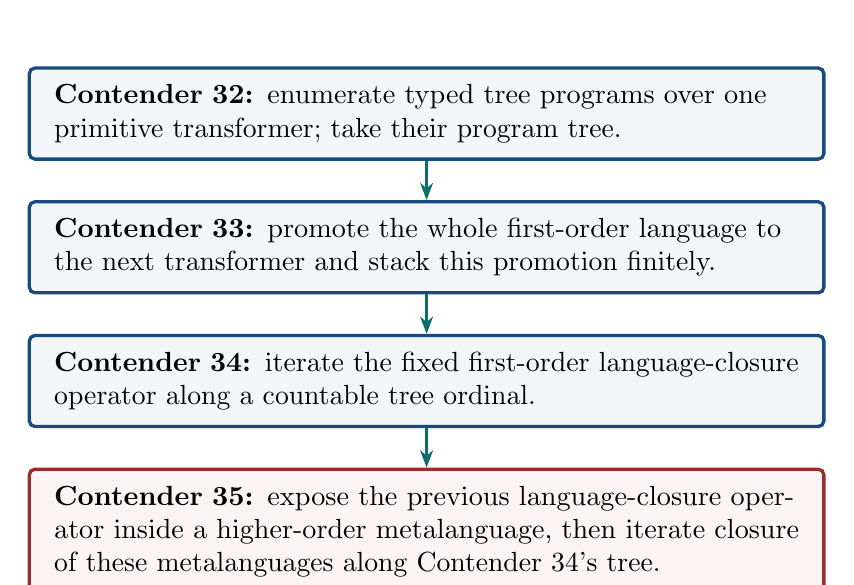
\begin{tikzpicture}[
  node distance=5mm,
  stagebox/.style={draw=BusyBlue, rounded corners=2pt, very thick,
    fill=BusyBlue!5, text width=0.78\textwidth, align=left,
    inner xsep=9pt, inner ysep=6pt},
  arrow/.style={-{Stealth[length=2.2mm]}, thick, draw=BusyTeal}
]
\node[stagebox] (c32) {\textbf{Contender 32:} enumerate typed tree programs over
one primitive transformer; take their program tree.};
\node[stagebox, below=of c32] (c33) {\textbf{Contender 33:} promote the whole
first-order language to the next transformer and stack this promotion finitely.};
\node[stagebox, below=of c33] (c34) {\textbf{Contender 34:} iterate the fixed
first-order language-closure operator along a countable tree ordinal.};
\node[stagebox, below=of c34, draw=BusyRed, fill=BusyRed!5] (c35)
{\textbf{Contender 35:} expose the previous language-closure operator inside a
higher-order metalanguage, then iterate closure of these metalanguages along
Contender 34's tree.};
\draw[arrow] (c32) -- (c33);
\draw[arrow] (c33) -- (c34);
\draw[arrow] (c34) -- (c35);
\end{tikzpicture}
\caption{The proposed step changes the functional type of the closure rule,
not only its iteration height.}
\label{fig:progression}
\end{figure}

\section{The incumbent and the design target}

\subsection{What Contender 34 already does}

Let
\[
  \Op = \CTree\to\CTree
\]
be the type of countable-tree transformers.  The accepted construction defines
\code{langLift} of type \(\Op\to\Op\).  Informally,
\(\Lang(b)(t)\) is the limit of \(P(t)\) over all closed, well-typed programs
\(P:\CTree\to\CTree\) in a simply typed language whose distinguished primitive
is the transformer \(b\).

Contender~33 iterates \(\Lang\) a finite number of times.  Contender~34 replaces
that finite iteration count by a countable tree ordinal.  In schematic form,
\[
\begin{aligned}
  B_0 & = \mathsf{boost}_{31},\\
  B_{a+1} & = \Lang(B_a),\\
  B_{\lim f}(t) & = \lim_i B_{f(i)}(t).
\end{aligned}
\]
At input \(n\), the height and argument are both a tree inherited from
Contender~33.  The numerical layer then reflects programs over addresses in
that tree and applies BusyLean's W-ranked hyperreflection.

This is already far beyond a hand-written ordinal notation.  Nevertheless,
there is a clear type-theoretic ceiling: throughout the construction,
\(\Lang\) is a fixed meta-level function.  Object-language programs can apply
the current tree transformer, but cannot receive a language-closure operator
as data and apply it to a transformer they have computed.

\subsection{Requirements for a genuine successor}

A serious successor should satisfy all of the following.

\begin{enumerate}[label=\textbf{R\arabic*.},leftmargin=3.2em]
  \item \textbf{Constructive closed natural.}  The final term must be a closed
  Lean \code{Nat}, with no oracle, noncomputable choice, unsafe implementation,
  partial definition, or opaque stand-in.

  \item \textbf{Formal strict comparison.}  A Lean theorem must prove
  \code{contender\_34 < contender\_35}.

  \item \textbf{No constant smuggling.}  The definition of
  \code{contender\_35} must not depend on the constant
  \code{contender\_34}.  It may use the previous construction as a family, as
  BusyLean's rules permit.

  \item \textbf{Qualitative increase.}  The new machinery should increase the
  expressive type of the closure operation, not only enlarge a numeric
  parameter or repeat the exact same reflection one more time.

  \item \textbf{Small trusted base.}  The extension should reuse the existing
  normalization, address well-foundedness, and W-ranked lift theorems rather
  than adding an unverified ordinal comparison or a new axiom.

  \item \textbf{Kernel tractability.}  Definitions and comparison proofs must
  elaborate without evaluating the represented number or enumerating the huge
  program lists.
\end{enumerate}

The construction below was chosen to meet these requirements simultaneously.

\section{The functional-type jump}

\subsection{Two operator levels}

Write
\[
  T = \CTree,
  \qquad
  \Op = T\to T,
  \qquad
  \MOp = \Op\to\Op.
\]
The first-order language closure has type
\[
  \Lang : \MOp.
\]
Contender~34 iterates this particular element of \(\MOp\) along a tree.  The
new idea is to define a closure operation on \emph{arbitrary elements of
\(\MOp\)}:
\[
  \MetaLang : \MOp\to\MOp.
\]
Thus a successor step no longer says merely ``close under all programs using
this tree transformer.''  It says ``close under all programs that can use both
this tree transformer and the previous \emph{closure operator}.''

The distinction is the same structural distinction that separates a hierarchy
of functions from a hierarchy of functionals acting on that hierarchy.  It is
not an exact ordinal analysis, but it is a robust reason to expect a major
increase in definability and growth.

\subsection{Why the new primitive is first-class enough}

The metalanguage adds the constructor
\begin{lstlisting}
| lift : Tm Gamma (.arr .tree .tree) ->
    Tm Gamma .tree -> Tm Gamma .tree
\end{lstlisting}
with semantic interpretation
\begin{lstlisting}
| .lift b t, rho =>
    liftF (b.eval liftF boostF rho) (t.eval liftF boostF rho)
\end{lstlisting}
Although \code{lift} is presented as a primitive constructor, ordinary lambda
abstraction makes the corresponding functional available as a value.  For
example, the term
\[
  \lambda b:T\to T.\;\lambda t:T.\;\mathsf{lift}\;b\;t
\]
has type \((T\to T)\to T\to T\).  Programs may pass such functionals to
higher-order combinators, iterate them by natural recursion, and use them in
tree recursion at arbitrary simple types.

The calculus remains predicative and simply typed.  There is no type of all
types, no impredicative self-encoding, and no general recursion.  In
particular, this proposal does not rely on a normalization conjecture: its
interpreter is a structurally recursive Lean definition.

\section{Syntax, typing, and total semantics}

\subsection{Reusing the existing type universe}

The metalanguage reuses the three type constructors from the existing tree
language:
\[
  A,B ::= \mathsf{nat}\mid\mathsf{tree}\mid A\to B.
\]
Their denotations are Lean's \code{Nat}, the repository's \code{CTree}, and
ordinary Lean function spaces.  Variables are intrinsically typed de Bruijn
indices.  Consequently, every constructor of \code{MTL.Tm Gamma A} denotes a
Lean value of the interpretation of \(A\).

The term constructors are:
\begin{itemize}[leftmargin=2em]
  \item variables, lambda abstraction, and application;
  \item zero, successor, and primitive recursion on naturals;
  \item zero, successor, and countable limit for trees;
  \item structural recursion over trees at any simple result type;
  \item \code{boost : tree -> tree};
  \item \code{lift : (tree -> tree) -> tree -> tree}.
\end{itemize}

\subsection{Semantic evaluation}

For a closure operator \(L\in\MOp\) and a base transformer \(b\in\Op\), the
interpreter has type
\[
  \mathsf{eval}_{L,b} : \mathsf{Tm}(\Gamma,A)
      \to \llbracket\Gamma\rrbracket\to\llbracket A\rrbracket.
\]
Every recursive call is made on a strict subterm, except for calls to the
already-total natural and tree iterators.  The two distinguished cases are
\[
\begin{aligned}
  \llbracket\mathsf{boost}\;t\rrbracket_{L,b}
    &= b(\llbracket t\rrbracket_{L,b}),\\
  \llbracket\mathsf{lift}\;p\;t\rrbracket_{L,b}
    &= L(\llbracket p\rrbracket_{L,b})
         (\llbracket t\rrbracket_{L,b}).
\end{aligned}
\]
This makes totality transparent.  A program cannot loop by applying
\code{lift}; it can only invoke the total semantic function supplied as
\code{liftF}.

\begin{proposition}[Constructive evaluation]
For every closed well-typed metalanguage term \(p:A\), every total
\(L\in\MOp\), and every total \(b\in\Op\), the Lean expression
\(\mathsf{eval}_{L,b}(p)\) reduces in principle to a value of
\(\llbracket A\rrbracket\).
\end{proposition}

\begin{proof}
The evaluator is accepted by Lean's structural termination checker.  Natural
and tree recursion are defined by structural recursion on their respective
inductive inputs.  Function values are ordinary total Lean functions.  No
classical choice or partial evaluator occurs.
\end{proof}

\subsection{Raw terms and a decidable checker}

The package also supplies an untyped raw syntax.  Lambda nodes carry their
argument type, so inference is syntax-directed.  The checker returns either
\code{none} or a dependent pair \(\langle A,p\rangle\) with
\(p:\mathsf{Tm}(\Gamma,A)\).  Equality of simple types is decidable.  The new
case verifies that the first child has type \(T\to T\) and the second has type
\(T\):
\begin{lstlisting}
| .lift b r => do
    let <_, tb> <- infer Gamma b
    let <_, tr> <- infer Gamma r
    let tb' <- cast? (.arr .tree .tree) tb
    let tr' <- cast? .tree tr
    pure <.tree, .lift tb' tr'>
\end{lstlisting}
Here and below, ASCII angle-bracket notation in displayed excerpts stands for
Lean's dependent-pair brackets in the source file.

Because the output is intrinsically typed, checker soundness is built into its
result type.  There is no separate preservation theorem to trust at this
layer.

\subsection{Finite enumeration without evaluation at build time}

\code{rawsUpTo n} is a finite list of raw terms with construction depth at
most \(n\).  It extends the previous enumerator by the finite product
\[
  \{\mathsf{lift}(p,q): p,q\in\mathsf{rawsUpTo}(n-1)\}.
\]
Filtering this list through the checker and retaining closed terms of type
\(T\to T\) yields \code{MTL.funsUpTo}.  The definition is computable but is
not evaluated while Lean checks the module.  The enormous list remains under
lambda binders inside the tree representation.

\section{The metalanguage closure}

\subsection{Definition}

For \(L\in\MOp\), \(b\in\Op\), and \(t\in T\), define
\[
  \MetaLang(L)(b)(t)
  = \lim_{m\in\Nat}\;\lim_{i\in\Nat}
      P^{L,b}_{m,i}(t),
\]
where \(P^{L,b}_{m,i}\) is the \(i\)-th closed, checked metalanguage program of
type \(T\to T\) appearing in the finite enumeration of depth at most \(m\), or
the zero transformer when the index is out of range.

In Lean:
\begin{lstlisting}
def metaLangLift
    (liftF : (CTree -> CTree) -> CTree -> CTree)
    (b : CTree -> CTree) (t : CTree) : CTree :=
  .lim fun m => .lim fun i =>
    (((MTL.funsUpTo liftF b m)[i]?).map fun p => p t).getD .zero
\end{lstlisting}
The result is again an element of \(\MOp\) when the first argument is fixed:
\[
  \MetaLang : \MOp\to\MOp.
\]

\subsection{What one successor stage contains}

A single metalanguage closure contains, as branches, values of programs that
can perform all of the following before returning a tree:
\begin{enumerate}[leftmargin=2.3em]
  \item use zero, successor, and arbitrary countable limits;
  \item recurse along an input tree at any finite simple type;
  \item compose, iterate, and higher-order manipulate the base transformer
  \(b\);
  \item construct a new transformer \(q:T\to T\) inside the program;
  \item call the previous closure operator \(L(q)\) on a dynamically computed
  tree;
  \item nest such calls under natural recursion, tree recursion, lambdas, and
  higher-order applications.
\end{enumerate}

The fourth and fifth items are the crucial novelty.  In Contender~34 the
meta-level recursion decides in advance which transformer is promoted to the
next language.  Here a program can decide which transformer to promote as part
of its computation.

\subsection{Recovery of lower-level behavior}

Ignoring the \code{lift} constructor gives a syntax-preserving embedding of the
previous tree language into the metalanguage.  Under this embedding, evaluation
with base transformer \(b\) agrees with the previous evaluator.  Therefore the
new closure does not discard the first-order program universe; it contains it
and adds programs that invoke \(L\).

A fully formal syntactic embedding theorem would be a useful strengthening of
the package, but it is not needed for the strict numerical comparison.  The
current tree deliberately includes Contender~34's tree as branch zero, while
the numerical family is independently seeded with the whole Contender~34
family.

\section{Transfinite metalanguage iteration}

\subsection{Structural recursion on countable trees}

Define \(M_a\in\MOp\) by structural recursion on a countable tree \(a\):
\[
\begin{aligned}
  M_0 &= \Lang,\\
  M_{a+1} &= \MetaLang(M_a),\\
  M_{\lim f}(b)(t) &= \lim_{i\in\Nat} M_{f(i)}(b)(t).
\end{aligned}
\]
The repository's auxiliary \code{supL} and \code{supH} constructors use the
conservative base case \(\Lang\), matching the treatment in earlier tree
language modules.  Lean code:
\begin{lstlisting}
def metaBoostT : CTree -> (CTree -> CTree) -> CTree -> CTree
  | .zero => langLift
  | .succ a => metaLangLift (metaBoostT a)
  | .lim f => fun b t => .lim fun i => metaBoostT (f i) b t
  | .supL _ => langLift
  | .supH _ => langLift
\end{lstlisting}
Termination is inherited directly from the inductive structure of
\code{CTree}.  No comparison of ordinal codes is required.

\subsection{Self-height without circular definition}

At input \(n\), let
\[
  T_{34}(n)=\mathsf{treeStackedTree}(n).
\]
The new tree is
\[
  T_{35}(n)
  = \lim_i
  \begin{cases}
    T_{34}(n), & i=0,\\
    M_{T_{34}(n)}
      \bigl(B_{T_{34}(n)}\bigr)
      \bigl(T_{34}(n)\bigr), & i\ne0,
  \end{cases}
\]
where \(B_a=\mathsf{boostT}(a)\) is the first-order hierarchy from
Contender~34.

This is ``self-height'' only in the benign sense that a previously constructed
finite Lean value \(T_{34}(n)\) is used as an index and as an argument.  There
is no recursive equation in which \(T_{35}(n)\) occurs on its own right-hand
side.  Hence the definition remains ordinary structural recursion.

The exact Lean definition is:
\begin{lstlisting}
def metaLanguageTree (n : Nat) : CTree :=
  .lim fun i =>
    if i = 0 then treeStackedTree n
    else metaBoostT (treeStackedTree n)
      (boostT (treeStackedTree n)) (treeStackedTree n)
\end{lstlisting}

\begin{designprinciple}[Height, base, and argument all advance]
A weak successor could keep the same base transformer and merely increase the
iteration height.  The present construction advances all three inputs:
\(T_{34}(n)\) is the meta-iteration height, indexes the first-order base
hierarchy, and is the tree to which the resulting operator is applied.
\end{designprinciple}

\section{From a tree to a natural number}

\subsection{Address-ladder programs}

BusyLean already proves that strict descent through addresses of any
\code{CTree} is well-founded.  Applying its transfinite System-F ladder to
\(T_{35}(n)\) therefore gives a universe of atom types without a new ordinal
notation theorem.  The new module defines:
\begin{itemize}[leftmargin=2em]
  \item \code{sn\_erase\_metatree}: every accepted erased term over these
  addresses is strongly normalizing;
  \item \code{metavalue}: normalize a checked program relative to a packed
  natural-number oracle and decode its numeral;
  \item \code{metatreeLadderUpTo n}: the finite list of candidate programs at
  depth at most \(n\).
\end{itemize}

The value function is total because it carries the strong-normalization proof
required by the existing normalizer.  Ill-typed candidates return zero.

\subsection{Family-aware reflection}

For a family \(f_i:\Nat\to\Nat\), define
\[
\begin{split}
  R_{35}(\vec f,n) ={}& n+1 \\
  &+ \max\left(
      \max_{i\le n} f_i(n),
      \max_{p\in\mathcal P_n}
        \mathsf{metavalue}(n,\mathsf{pack}(\vec f),n,p)
    \right),
\end{split}
\]
where \(\mathcal P_n\) is the finite metalanguage-tree ladder.  The added
\(n+1\) makes strictness immediate even when one of the maxima is attained.

Lean packages this as \code{reflectMetaFamily} and the corresponding
\code{Transformer}.  Two elementary inequalities drive the comparison:
\begin{align*}
  i\le n &\implies f_i(n)<R_{35}(\vec f,n),\\
  p\in\mathcal P_n &\implies
    \mathsf{metavalue}(p)<R_{35}(\vec f,n).
\end{align*}
The first is exactly the progressiveness property required by BusyLean's
W-tree-ranked lift theorem.

\subsection{The seed, schedule, and rank}

Define the previous construction as a family rather than importing its final
constant:
\[
  \mathsf{family}_{34}(n)
    = \Fthirtyfour(\Fthirtyfour(n)).
\]
Then, definitionally,
\[
  \mathsf{family}_{34}(42)=\Cthirtyfour.
\]
The new schedule and rank are autonomous W-trees obtained by applying
\code{Autonomous.hyper} \(\mathsf{family}_{34}(n)+42\) times above the previous
schedule and then above the new schedule.  This preserves the architecture of
the accepted contender while enlarging both control trees by the full previous
family.

Finally,
\[
  \Fthirtyfive(n)
  = \mathsf{wDiagonalLift}
      (\mathsf{schedule}_{35}(n))
      (\mathsf{rank}_{35}(n))
      (\mathsf{metaTransformer})
      (\mathsf{family}_{34})\;n\;n,
\]
and
\[
  \boxed{\Cthirtyfive=\Fthirtyfive(\Fthirtyfive(42)).}
\]

\section{Formal comparison with Contender 34}

\subsection{The proof chain}

The comparison file proves the following sequence.

\begin{longtable}{>{\ttfamily}p{0.38\textwidth}p{0.55\textwidth}}
\toprule
\normalfont Theorem & Statement and role\\
\midrule
\endfirsthead
\toprule
\normalfont Theorem & Statement and role\\
\midrule
\endhead
lt\_reflectMetaFamily & Any number below the defining maximum is strictly below
\code{reflectMetaFamily}.\\
oracle\_lt\_reflectMetaFamily & Every visible seed coordinate is strictly
reflected.\\
metavalue\_lt\_reflectMetaFamily & Every enumerated program value is strictly
reflected.\\
metaTransformer\_progressive & The transformer satisfies the hypothesis of the
W-ranked lift theorem.\\
family34\_lt\_F35 & For every \(n\),
\(\mathsf{family}_{34}(n)<F_{35}(n)\).\\
raw\_meta\_reflection\_lt\_F35 & One raw reflection step is strictly below the
lifted hierarchy.\\
metavalue\_lt\_F35 & Every enumerated program value under the packed seed is
below \(F_{35}(n)\).\\
input\_lt\_family34 & \(n<\mathsf{family}_{34}(n)\).\\
input\_lt\_F35 & \(n<F_{35}(n)\).\\
contender\_34\_lt\_contender\_35 & The required final comparison.\\
\bottomrule
\end{longtable}

The final proof is only two strict transitivity steps:
\begin{lstlisting}
theorem contender_34_lt_contender_35 :
    contender_34 < contender_35 :=
  Nat.lt_trans (family34_lt_F35 42)
    (input_lt_F35 (F35 42))
\end{lstlisting}
The first term has left side
\(\mathsf{family}_{34}(42)=\Cthirtyfour\) by definitional reduction.  Its right
side is \(F_{35}(42)\).  The second term places \(F_{35}(42)\) below
\(F_{35}(F_{35}(42))=\Cthirtyfive\).

\subsection{Why this is not a disguised use of the previous constant}

The new definition imports \code{F34}, \code{schedule34}, and the reusable
constructional infrastructure.  It never mentions \code{contender\_34}.  The
audit computes the transitive constant dependency closure of
\code{contender\_35} and rejects the build if any contender constant from 5
through 34 occurs.

This distinction matters.  Writing \(C_{35}=C_{34}+1\) would be formally
larger but mathematically vacuous.  Writing
\(\mathsf{family}_{34}(n)=F_{34}(F_{34}(n))\) exposes the previous algorithm as
an oracle family to a stronger closure construction, which is the intended
BusyLean pattern.

\section{Constructive computability}

\subsection{Why the number exists as a computation}

Every component of the definition is constructive:
\begin{enumerate}[leftmargin=2.3em]
  \item raw terms up to a given depth form a finite recursively generated list;
  \item type inference is a terminating recursive function with decidable type
  equality;
  \item typed metalanguage evaluation is structural recursion;
  \item \code{metaLangLift} forms an inductive tree without enumerating all
  branches during elaboration;
  \item \code{metaBoostT} is structural recursion on a countable tree;
  \item addresses have a decidable well-founded descent relation;
  \item the existing System-F normalizer is total on terms equipped with its
  formal strong-normalization witness;
  \item finite maxima, family packing, autonomous W-tree realization, and the
  W-ranked lift are executable Lean definitions;
  \item the outer expression applies total functions to the numeral 42.
\end{enumerate}
Thus \code{contender\_35 : Nat} is computable in the ordinary recursion-theoretic
sense: a sufficiently idealized machine following Lean's evaluator eventually
returns a unary/binary representation of a natural number.  Feasibility is not
claimed.  As with prior BusyLean contenders, actually requesting the numeral is
prohibitive and unnecessary.

\subsection{No hidden nonconstructive shortcut}

The metalanguage module contains no \code{noncomputable}, \code{partial},
\code{unsafe}, \code{opaque}, \code{extern}, or custom axiom declaration.  Its
semantic function spaces are constructive Lean function types.  The proof
layer may inherit Lean's standard propositional extensionality and quotient
soundness through earlier modules, exactly within the repository's stated
allowance; the numerical definition itself does not become an oracle thereby.

\section{Why the increase is significant}

\subsection{Parameter growth versus type growth}

There are two fundamentally different ways to enlarge a hierarchy.

\paragraph{Parameter growth.}
Keep the same closure operator and use a larger finite count, ordinal index,
schedule, rank, or starting argument.  This can be enormous, but the class of
one-step closure rules is unchanged.

\paragraph{Type growth.}
Promote the closure operator to an argument available inside the language,
then close under programs that manipulate it.  New one-step rules become
definable because programs can synthesize a transformer and ask the previous
closure mechanism to close over it.

Contender~35 performs both, but the second is decisive.  It changes
\(\Lang\in\MOp\) from fixed metalogical infrastructure into an object-language
capability and then iterates the resulting operation
\(\MetaLang:\MOp\to\MOp\) transfinitely.

\subsection{A schematic separation example}

At a first-order stage, a program may use a distinguished transformer \(b\),
compose it, and recurse with it.  Which transformer is promoted by the next
\(\Lang\) step is fixed externally.

At a metalanguage stage, a program can compute a transformer
\[
  q_x(t)=\mathsf{treeRec}(\ldots,x,t)
\]
depending on run-time data \(x\), then form \(L(q_x)(u)\) inside the same
program.  It may repeat this under a transfinite tree recursion whose branches
select different \(q_x\).  The set of promoted languages is therefore itself
program-generated.

This is the operational content of the type jump.  It is stronger evidence
than a decorative increase in the numeral 42 or one extra use of the existing
lift.

\subsection{Four amplifications are composed}

The final number combines four distinct amplifiers:
\begin{enumerate}[leftmargin=2.3em]
  \item all closed metalanguage programs at all finite sizes;
  \item transfinite iteration of metalanguage closure to height
  \(T_{34}(n)\);
  \item reflection over all bounded System-F ladder programs whose atoms are
  addresses of the resulting tree;
  \item W-tree-ranked iteration over schedules and ranks expanded using the
  entire previous family.
\end{enumerate}
Any one of these would yield a larger construction.  Their composition is why
Contender~35 is intended as a serious successor rather than an incremental
patch.

\subsection{What is and is not proved}

The Lean theorem proves the exact natural-number inequality
\(C_{34}<C_{35}\).  The source also proves uniform domination of
\(\mathsf{family}_{34}(n)\) by \(F_{35}(n)\), plus bounds for every enumerated
metalanguage-tree program.

It does \emph{not} prove an exact fast-growing-hierarchy index or a strict
ordinal inequality between the semantic ranks of \(T_{34}(n)\) and
\(T_{35}(n)\).  Assigning proof-theoretic ordinals to languages with these
higher-order semantic closure operators would itself be a substantial research
project.  The report therefore describes the growth-rate jump as a structural
and type-theoretic argument, not as a completed ordinal analysis.

\section{Safety, predicativity, and consistency posture}

\subsection{No self-interpreter}

A tempting but dangerous route would be to encode the metalanguage's own syntax
and evaluator inside itself, then diagonalize.  Such a construction would need
a delicate normalization or consistency proof and could accidentally introduce
a partial evaluator.  The present proposal does not do this.

The semantic parameter \code{liftF} is supplied from Lean's metalanguage.  A
program can call it only through a typed primitive.  It cannot inspect its code,
modify its evaluator, or form an untyped self-application.

\subsection{Predicative simple types}

All types are generated from \code{nat} and \code{tree} by the arrow
constructor.  There is no universe object containing all simple types and no
quantification over the totality to which the current type belongs.  Higher
functionals arise from finite arrow nesting, and transfinite iteration is over
an inductive tree.  This keeps the new module within the same conservative
semantic style as the accepted tree-language modules.

\subsection{Fallback constructors}

The repository's \code{CTree} has constructors \code{supL} and \code{supH}
used by earlier collapsing machinery.  The previous \code{boostT} maps these to
the base transformer, rather than attempting a new recursion principle over
their payloads.  \code{metaBoostT} follows the same convention, returning
\code{langLift}.  This makes the extension compatible with the established
structural-recursion boundary.

\section{Verification and audit protocol}

\subsection{Exact environment}

The package targets the repository's pinned toolchain, Lean~4.34.0, and its
existing Lake dependency graph.  Verification is designed to run after the
accepted Contender~34 modules are precompiled, matching the contest's rule that
historical contenders may be cached.

\subsection{Checks performed}

The isolated audit performs four classes of checks:
\begin{enumerate}[leftmargin=2.3em]
  \item kernel elaboration of \code{TreeLanguage4}, \code{Contender35}, and
  \code{Comparison35};
  \item \code{\#print axioms} on the evaluator, the closure operators, the new
  number, the comparison theorem, and the program-value bound;
  \item transitive dependency-closure rejection of all constants
  \code{contender\_5} through \code{contender\_34};
  \item timing of the three new module builds without evaluating the number.
\end{enumerate}

\subsection{Verification status}

\StatusText

The archive includes \code{VERIFICATION.md} and machine-readable/log artifacts
recording the exact commit, workflow run, diagnostics, timings, and axiom
output.  They provide the complete reproducible record of the successful check.

\section{Integration into BusyLean}

The proposal is deliberately modular.  Integration requires adding the
following imports after Contender~34:
\begin{lstlisting}
import BusyLean.Ordinal.TreeLanguage4
import BusyLean.Contender35
import BusyLean.Comparison35
\end{lstlisting}
The supplied integration script copies the three modules and the audit into an
existing checkout.  The main repository audit should then add
\code{\#print axioms} commands for the new declarations and an
\code{\#assert\_not\_in\_closure} block for \code{contender\_35}.  The check
script's \code{PREVIOUS} module should move from \code{Comparison33} or
\code{Comparison34}, as appropriate to its current organization, to
\code{Comparison34}, while the timed definition/proof targets become the new
modules.

No change to earlier accepted definitions is required.  The proposal can be
reviewed as a three-module extension.

\section{Alternative designs considered}

\subsection{Another tree-ordinal stacking round}

One could define a larger height such as
\(\mathsf{boostT}(T_{34})(T_{34})\) and otherwise copy Contender~34.  This is
constructive and easy to compare, but remains within the same first-order
operator \(\Lang\).  It would be a parameter increase, not a new closure
principle.

\subsection{A second W-ranked lift only}

One could nest \code{wDiagonalLift} around \(F_{34}\) with larger schedules and
ranks.  This would certainly dominate the seed, but would leave the reflected
object language unchanged.  The present proposal retains the stronger schedule
and rank while also changing the language layer.

\subsection{Untyped universal interpreters}

Enumerating arbitrary Lean programs or Turing machines would permit a dramatic
diagonal, but totality would become undecidable.  Bounding execution by fuel
would restore computability at the cost of turning the construction into a
resource-bound busy-beaver surrogate, contrary to the repository's proof-
theoretic style.  The typed semantic language gives a totality certificate by
construction.

\subsection{Impredicative language universes}

A universe whose elements include its own closure operator could promise still
larger strength.  It would require a new reducibility or model construction and
would risk a Girard-style circularity.  A one-level predicative metalanguage is
a safer and already substantial advance.

\section{Further research program}

\subsection{Formal embedding and rank theorems}

The most immediate strengthening is to formalize the embedding of the previous
\code{TL} language into \code{MTL}.  Desirable theorems include:
\begin{align*}
  \mathsf{eval}_{\mathrm{MTL}}(\iota p,L,b)
    &= \mathsf{eval}_{\mathrm{TL}}(p,b),\\
  \mathsf{programTree}(b,m)
    &\preccurlyeq \mathsf{metaLangLift}(L,b,t)
    \quad\text{for an explicit branch embedding.}
\end{align*}
One can then seek address embeddings between \(T_{34}(n)\) and
\(T_{35}(n)\), not merely inclusion as branch zero.

\subsection{All finite meta-levels}

Define recursively
\[
  \Op_0=T\to T,
  \qquad
  \Op_{k+1}=\Op_k\to\Op_k.
\]
Contender~35 uses level one.  A family of intrinsically typed languages could
make \(k\) an input and close over operators at every finite level.  The main
technical issue is representing the denotation of \(\Op_k\) without making
Lean elaborate infeasibly large dependent terms.

\subsection{Tree-indexed functional levels}

A more ambitious extension would replace the natural level \(k\) by a tree
ordinal and define a dependent family of functional types with products at
limits, paralleling Contender~31's transfinite closure types.  The language
would then manipulate closure operators whose \emph{types} are indexed by the
same tree used for iteration.

\subsection{A typed code universe with certified evaluation}

Instead of external finite enumeration, one could add a predicative code type
for metalanguage terms and a total evaluator whose termination is proved by a
logical relation.  Programs could construct certified codes dynamically.  The
challenge is avoiding a self-code that invalidates stratification.

\subsection{Exact proof-theoretic calibration}

The hierarchy appears related to autonomous progressions of reflection
principles and higher-type recursion over well-founded trees.  A serious
calibration would require:
\begin{enumerate}[leftmargin=2.3em]
  \item a theory whose provably total functionals match the metalanguage
  stages;
  \item a notation/collapse system for its reflection closure;
  \item upper and lower simulations between that theory and the Lean
  definitions;
  \item a comparison with the W-ranked numerical amplifier.
\end{enumerate}
Until such work is done, exact ordinal labels should be treated as conjectural.

\subsection{Performance engineering}

The raw enumerator intentionally repeats many terms.  A semantics-preserving
quotient by type, size, and alpha-equivalence could greatly reduce small smoke
tests.  More importantly, the proof modules should remain insensitive to the
enumeration's actual size: no command should force evaluation beyond tiny
examples.  Automated checks can inspect reducibility traces and generated code
to guard against accidental evaluation.

\section{Conclusion}

Contender~35 is designed as the next conceptual step after languages stacked
along tree ordinals.  It promotes the language-closure operator to a typed
primitive, closes under programs that manipulate that operator, and iterates
the resulting metalanguages along Contender~34's own tree.  The construction is
predicative, total by structural recursion, and compatible with BusyLean's
existing normalization and W-tree reflection infrastructure.

The exact theorem \(C_{34}<C_{35}\) follows from uniform family domination and
strict inflationarity.  The more ambitious claim---that the number is not just
larger but belongs to a substantially stronger growth regime---is supported by
the one-functional-type jump and the transfinite closure architecture.  The
package avoids pretending that this structural evidence is already an exact
ordinal analysis.

\appendix
\section{Complete Lean source: the metalanguage}
\label{app:tree-language-four}
\lstinputlisting{../BusyLean/Ordinal/TreeLanguage4.lean}

\section{Complete Lean source: the number}
\label{app:contender-thirty-five}
\lstinputlisting{../BusyLean/Contender35.lean}

\section{Complete Lean source: comparison theorems}
\label{app:comparison-thirty-five}
\lstinputlisting{../BusyLean/Comparison35.lean}

\section{Artifact map}

\begin{longtable}{p{0.43\textwidth}p{0.50\textwidth}}
\toprule
Artifact & Purpose\\
\midrule
\endfirsthead
\toprule
Artifact & Purpose\\
\midrule
\endhead
\code{BusyLean/Ordinal/TreeLanguage4.lean} & Typed metalanguage,
interpreter, checker, enumeration, closure, and transfinite iteration.\\
\code{BusyLean/Contender35.lean} & Address-ladder value function, family
reflection, schedule, rank, \(F_{35}\), and the closed number.\\
\code{BusyLean/Comparison35.lean} & Progressiveness, program bounds,
uniform family domination, and final comparison.\\
\code{test/Contender35Audit.lean} & Axiom reports and forbidden-constant
closure check.\\
\path{article/contender35_metalanguage.tex} & Source of this report.\\
\path{article/contender35_metalanguage.pdf} & Compiled report.\\
\code{VERIFICATION.md} & Exact kernel-check status, diagnostics, timings, and
workflow identifiers.\\
\code{apply\_to\_checkout.sh} & Idempotent integration helper.\\
\code{MANIFEST.sha256} & Integrity hashes for packaged artifacts.\\
\bottomrule
\end{longtable}

\begin{thebibliography}{9}

\bibitem{GoedelT}
Kurt G\"odel.
\newblock {\"U}ber eine bisher noch nicht ben\"utzte Erweiterung des finiten
Standpunktes.
\newblock \emph{Dialectica}, 12:280--287, 1958.

\bibitem{TaitComputability}
William W. Tait.
\newblock Intensional interpretations of functionals of finite type I.
\newblock \emph{Journal of Symbolic Logic}, 32(2):198--212, 1967.

\bibitem{GirardProofsTypes}
Jean-Yves Girard, Yves Lafont, and Paul Taylor.
\newblock \emph{Proofs and Types}.
\newblock Cambridge University Press, 1989.

\bibitem{FefermanProgressions}
Solomon Feferman.
\newblock Transfinite recursive progressions of axiomatic theories.
\newblock \emph{Journal of Symbolic Logic}, 27(3):259--316, 1962.

\bibitem{HowardOrdinalAnalysis}
William A. Howard.
\newblock Ordinal analysis of terms of finite type.
\newblock \emph{Journal of Symbolic Logic}, 45(3):493--504, 1980.

\bibitem{Lean4}
Leonardo de Moura and Sebastian Ullrich.
\newblock The Lean 4 theorem prover and programming language.
\newblock In \emph{Automated Deduction---CADE 28}, pages 625--635, 2021.

\bibitem{BusyLean}
Vladimir Reshetnikov.
\newblock \emph{BusyLean: name the biggest number, in Lean}.
\newblock Repository documentation and formal source, consulted 13 October
2026.

\end{thebibliography}

\end{document}
